%**************************************************************
\subsubsection{Package it.tecsen.smacs.screen}
\label{subsubsec:it-tecsen-smacs-screen}

% L'immagine dovrebbe essere qui ma per motivi di spazio viene spostata.
In questo package vi sono tutte le classi che implementano i widget radice di ogni schermata dell'applicazione, come è stato precedentemente illustrato in "\hyperref[subsubsec:it-tecsen-smacs]{Package it.tecsen.smacs}".\\
Ogni screen implementa uno o più casi d'uso, disponibili per la consultazione nell'appendice "\hyperref[cap:analisi-dei-requisiti]{Analisi dei requisiti}".
% \\
\clearpage
\begin{figure}[!h]
  \centering 
  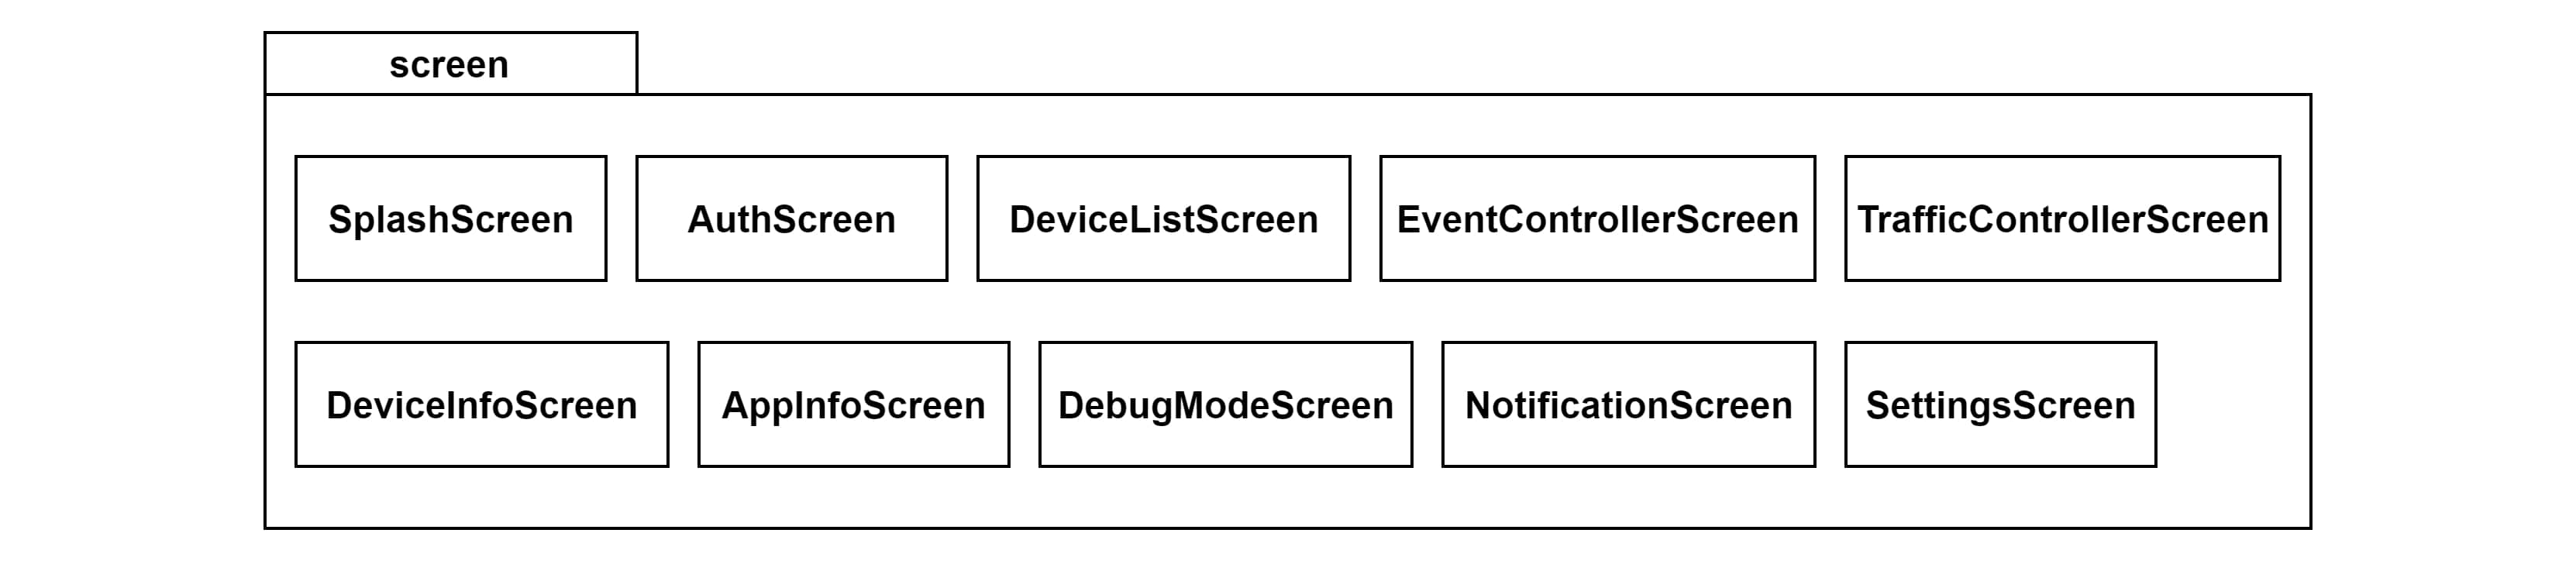
\includegraphics[width=1.0\columnwidth]{capitolo-6/organizzazione-package/screen} 
  \caption{Diagramma del package \texttt{it.tecsen.smacs.screen}}
\end{figure}
In particolare:
{
\renewcommand{\arraystretch}{1.5}
\begin{longtable}{|c|c|}
    \hline
    \textbf{Classe (widget)} & \textbf{Caso (e sotto-casi) d'uso implementati} \\\hline
    \endhead
    SplashScreen & UC01\\\hline
    AuthScreen & UC02 \\\hline
    DeviceListScreen & UC03, UC15 \\\hline
    TrafficControllerScreen & UC04, UC05, UC07, UC09, UC10 \\\hline
    DeviceInfoScreen & UC06 \\\hline
    EventControllerScreen & UC08 \\\hline
    NotificationScreen & UC11 \\\hline
    SettingsScreen & UC12 \\\hline
    AppInfoScreen & UC13 \\\hline
    DebugModeScreen & UC14 \\\hline
    \caption{Correlazione fra classi del package \texttt{screen} e casi d'uso implementati}
\end{longtable}
}
